\chapter{Generalization}

In this chapter we show how to make the algorithm more 
abstract by allowing flexibilty through functions as parameters and
finding minimal requirements for the data-structures.

\section{Algorithm}

The algorithm in a more convetional view is:

\begin{algorithm}[H]
	\caption{The SPEXS2 algorithm}
\begin{algorithmic}[1]
	\Require{$dataset$, $in$ pool, $out$ pool, $extender$,
		$extendable$ filter, $outputtable$ filter, $postprocess$ function }
	\Ensure{Patterns satisfying filters and $extender$ are in $out$ pool}
	\Statef{\varepsilon \gets NewEmptyQuery(dataset)}
	\Statef{in.put(\varepsilon)}
	\While{$q \gets in.take()$}
		\Statef{extended \gets extender(q, dataset)}
		\For{ $qx \in extended$ }
			\If{ $extendable(qx)$ }
				\Statef{in.put(qx)}
			\EndIf
			\If{ $outputtable(qx)$ }
				\Statef{out.put(qx)}
			\EndIf
		\EndFor
		\Statef{postprocess(q)}
	\EndWhile
\end{algorithmic}
\end{algorithm}

When the algorithm starts we create an empty pattern query and put 
into the in pool. The in pool contains queries whose patterns
should be further examined.

We pick a query from the in pool for extending. The extending means
generating all queries whose pattern is larger by one. There can be
several such queries.

If any of the queries should be further examined as defined by the
extendable filter, it will be put into the in pool.

If the query is fit for output we as defined by the outputtable filter,
it will be put into the out pool.

If we extend each pattern at each step by one we guarantee that we
examine the all patterns that conform to our criteria.

\section{Pools}

Pool is an abstract datatype for a collection of queries. The pool
allows queries to be put into it and taken from it, also we can
ask whether the pool is empty or not.

It has no guarantees on how the queries are stored internally and
in which order they are taken out.

In practice this means we can use any collection such as list, set,
queue as a pool. This gives us different performance characteristics.

This also means that pools can persist the queries if necesssary.

\section{Filtering}

Filtering allows us to dramatically reduce the number of queries
we have to look at. It also allows to select only interesting patterns by
some criteria.

If we have interestingness measure we can create filter from it by
defining it's minimum or maximum value. One very usefule example 
would be a filter for limiting the pattern length.

By separating the extension and output filter, as opposed to SPEXS, 
we can still limit output without affecting the extension process.
For example if we wish to see only patterns of length 3 we cannot do
it with one filter. Since we need to extend patterns of length 0, 1 and 2.

\section{Extending}

The extending process is at the core of the algorithm. 
We shall look at how we can deal with different types.

The extending method is:

\begin{algorithm}[H]
	\caption{SPEXS2 extender}
\begin{algorithmic}[1]
	\Require{$q$ query, $next$ function}
	\Ensure{result contains queries that have been extended by one}
	
	\Statef{nexts \gets new~collection}
	\For{$pos \in matches(q)$}
		\Statef{(token, pos) \gets next(pos)}
		\Statef{nexts.put((token, pos))}
	\EndFor

	\Statef{matches \gets new~map~of~token~to~position~set }
	\For{$(token, pos) \in nexts$}
		\If{$matches[token]$ doesn't exist}
			\Statef{matches[token] \gets \{\} }
		\EndIf
		\Statef{matches[token] \gets matches[token] + \{pos\} }
	\EndFor

	\Statef{result \gets new~collection}
	\For{$(token, positions) \in matches$}
		\Statef{qx \gets new~query}
		\Statef{qx.pattern \gets q.pattern + token}
		\Statef{qx.positions \gets positions}
		\Statef{result.add(qx)}
	\EndFor
\end{algorithmic}
\end{algorithm}

This extender depends on how next is implemented, we shall look at different
ways how to implement it.

\subsection{Sequences}

The simplest case how the next function behaves is when we are only looking for simple sequences.

Let's consider a sequence ACGCCGATCGC and a pattern CG.

Diagram of the ACG.CCG.ATCG.C and query for that pattern.

Next positions step is finding ACG.[C]CG.[A]TCG.[C].

Grouping is [C] ==> CGC, [A] => CGA.

\begin{figure}[H]
	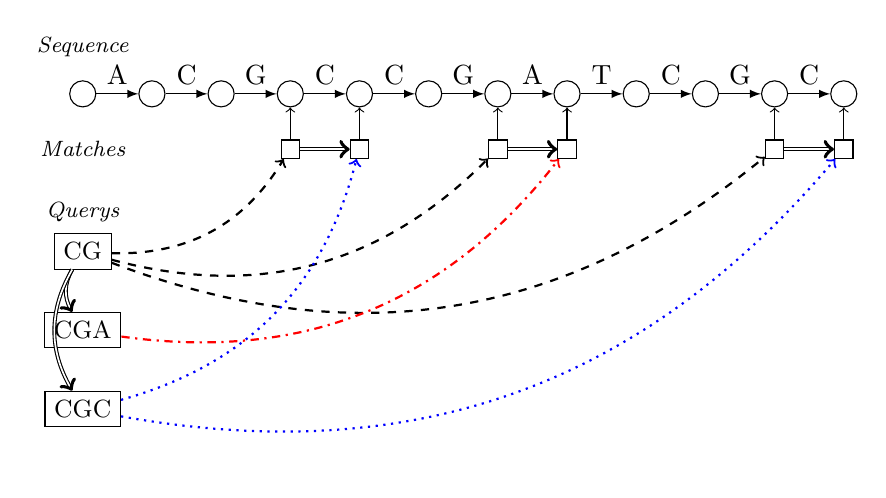
\begin{tikzpicture}[auto]
	\tikzstyle{state} = [ draw, circle, thin, node distance = 2.5em, font={\small}];
	\tikzstyle{query} = [ draw, rectangle, thin, node distance = 2.5em, font={\small}];
	\tikzstyle{info} = [font={\itshape\footnotesize}]
	\tikzstyle{point}  = [ ->, thin, font={\small}];
	\tikzstyle{extend} = [ ->, double, font={\small}];
	\tikzstyle{trace} = [ ->, thick, dashed, bend right, font={\small} ];

	\def \seq {X,A,C,G,C,C,G,A,T,C,G,C}

	\foreach \x [count=\xi] in \seq {
		\ifnum 1 < \xi
			\pgfmathparse{int(\xi-1)}
			\let \li \pgfmathresult
			\node[state, right of=\li] (\xi) {};
			\draw[->, >=latex] (\li) to node{\x} (\xi);
		\else
			\node[state] (\xi) {};
		\fi
	}

	\node[info] at (0,0.6) {Sequence};
	\node[info] at (0,-0.7) {Matches};
	\node[info] at (0,-1.5) {Querys};

	\node[query](CG)  at (0,-2) {CG};
	\node[query](CGA) at (0,-3) {CGA};
	\node[query](CGC) at (0,-4) {CGC};

	\tikzstyle{traceCG} = [ ->, thick, dashed, bend right, color=black ];
	\tikzstyle{traceCGA} = [ ->, thick, dashdotted, bend right, color=red ];
	\tikzstyle{traceCGC} = [ ->, thick, dotted, bend right, color=blue ];

	\draw[extend, bend right] (CG) to (CGA);
	\draw[extend, bend right] (CG) to (CGC);

	\foreach \xi/\xv in {4/CG,7/CG,11/CG} {
		\node[draw, below of=\xi, node distance=2em] (p\xi) {};
		\draw[point] (p\xi) to (\xi);
		\draw[trace\xv] (\xv) to (p\xi);
	}

	\foreach \xi/\xv in {5/CGC,8/CGA,12/CGC} {
		\node[draw, below of=\xi, node distance=2em] (p\xi) {};
		\draw[point] (p\xi) to (\xi);
		\draw[trace\xv] (\xv) to (p\xi);
	}

	\foreach \xi/\yi in {4/5,7/8,11/12} {
		\draw[extend] (p\xi) to (p\yi);
	}
\end{tikzpicture}

\end{figure}

\subsection{Groups and Stars}

Since we want to find more interesting patterns we can add more
information to the sequence DFA. Such as a star expression.

Same sequence with star paths.

\missingfigure{sketch of more complex}

\subsection{Optimizations}

Although we can add the group information to the DFA, it is more
performant to use the information gathered from the extension
of non-groups.

A[CG].Positions = AC.Positions union AG.Positions

\missingfigure{sketch of possible optimizations}

\subsection{Other}

There maybe several other extensions to the regular expressions.

Questionable position:

AC?.Positions = A.Positions + AC.Positions

\missingfigure{sketch of questions}